\documentclass[a4paper, 12pt]{article}

\usepackage[utf8]{inputenc}

%images
\usepackage{graphicx}       %for inserting images
\graphicspath{./images/}    %image file directory
\usepackage{wrapfig}
%caption
\usepackage{caption}
\captionsetup{
   font=small,
   labelfont=bf,
   tableposition=top
}
%page margins, geometry
\usepackage{geometry}
\geometry{margin = 1in}

%headers and footers
% All page numbers positioned at the bottom of the page
\usepackage{fancyhdr}
\fancyhf{} % clear all header and footers
\fancyfoot[C]{\thepage}
\renewcommand{\headrulewidth}{0pt} % remove the header rule
\pagestyle{fancy}

%for inserting columns
\usepackage{multicol}       
\setlength{\columnsep}{1cm}

%bibilography
\usepackage{biblatex}
\addbibresource{biblography.bib}

%to use sample texts
\usepackage{blindtext}


\begin{document}
\fancyhead[l]{EN2532 - Robot Design and Competition}
\fancyhead[r]{Group BASC}
\begin{flushleft}
     \textsc{\Huge {Assignment 6 \\}}
\end{flushleft}


%document authors 
\begin{center}
\begin{tabular}{c c c c}
     \textsc{Y.S. Ginige} & 180195A &  \textsc{P.M.P.H. Somarathne} & 180616T\\
     \textsc{V.Y.N. Lokugama }& 180359G & \textsc{A. Thieshanthan} &  180641N\\
       \textsc{W.A.V. Ravihansa} &  180544U &  \textsc{L.T.N. Wickremasinghe} & 180701B
\end{tabular}
\end{center}


%content after this

\normalsize
\section*{Question 1}
    \begin{figure}[h]
        \centering
        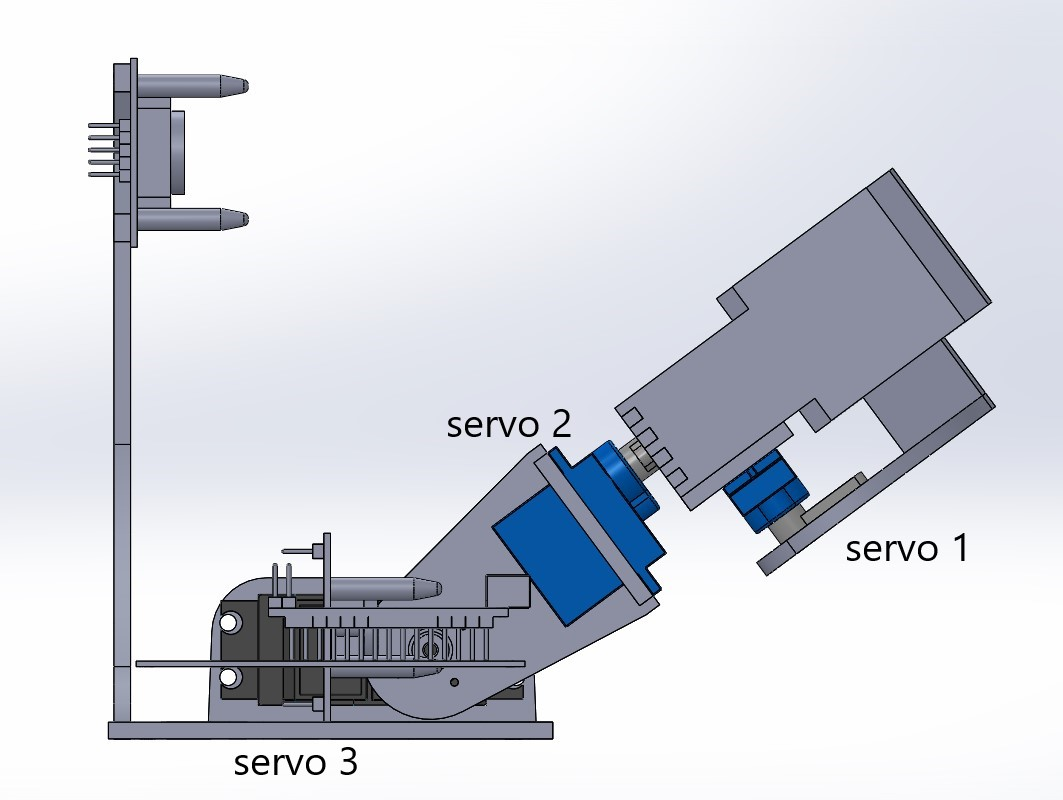
\includegraphics[scale = 0.4]{images/side arm.jpg}
        \caption{Side view  of arm}
        \label{fig:side}
    \end{figure}
        $
            weight\_of\_box = 0.100kg \\
            weight\_of\_servo1 = w_1 \\
            distance\_to\_servo1 = 5.6cm \\
            weight\_of\_servo2 = w_2 \\
            distance\_to\_servo2 = 3.1cm \\
            weight\_of\_gripping\_parts = 0.200kg \\
            distance\_to\_box = 9cm \\
            distance\_to\_gripper = 5.6cm \\
            \\
            Torque\_required\_for\_servo3 = 0.1 \times 8 + 0.2  \times 5.6 + w_1 \times 5.6 + w_2 \times 3.1
            \\
            Torque\_for\_servo1 = 0.05 \times 2.3  = 0.115 kgcm \\$
            
        
        
    With these calculations Tower pro SG90 Servo Motor can be used for servo1 and servo2. Which will set $w_1 = w_2 = 0.0147kg$. Then,\\
    \\
    $Torque\_required\_for\_servo3 = 0.1 \times 8 + 0.2  \times 5.6 + 0.0147 \times 5.6 + 0.0147 \times 3.1 = 2.047 kgcm$ \\
    To have 50\% cushion for errors Tower Pro SG5010 can be used for servo3.
    % \begin{figure}[h]
    %     \centering
    %     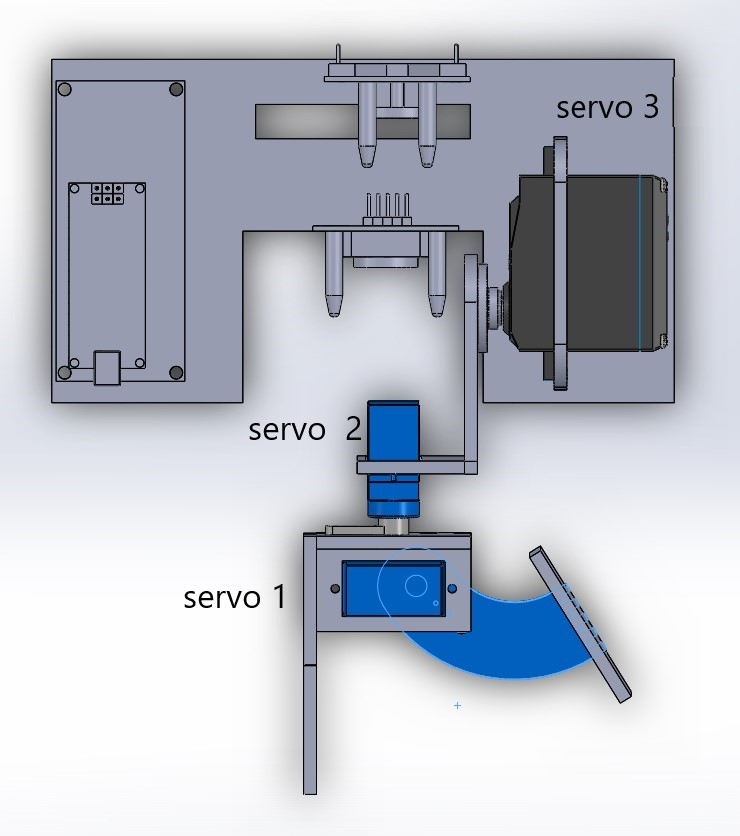
\includegraphics[scale = 0.3]{images/top arm.jpg}
    %     \caption{Side view  of arm}
    %     \label{fig:side}
    % \end{figure}

\section*{Question 2 - PID algorithm for line following}
    \subsection*{Global variables}
        $Error \longleftarrow 0\\
        prevError \longleftarrow 0\\
        deltaError \longleftarrow 0\\
        sumError \longleftarrow 0\\
        Kp \longleftarrow x\\
        Kd \longleftarrow y\\
        Ki \longleftarrow z\\
        leftBaseSpeed \longleftarrow lb\\
        rightBaseSpeed \longleftarrow rb\\
        positiveMax \longleftarrow m\\
        negativeMax \longleftarrow n\\
        PIDpositiveMax \longleftarrow p\\
        PIDnegativeMax \longleftarrow q\\$\\
        
        Initializing the variables Error, prevError, deltaError, sumError to hold the values that will be updated each time getPID() function is called.
        \par
        The Kp, Ki, and Kd values will be the tuning parameters of the PID control.
        The base speed is the speed of motors the drive the wheels of the robot when the body is in line with no error.
        It will be a good idea to define two base speeds to the two motors since motors may not behave identically.
        positiveMax and negativeMax will be the bounds we set for the speed of the motor.
        \par
        PIDpositiveMax and PIDnegativeMax will be the bounds we set for the output of the getPID() function.


    \subsection*{Basic structure of line follower code}
        $Repeat \\ \{\\
        \indent      pidVal \longleftarrow  getPID()\\
         \indent           LeftMotorSpeed \longleftarrow  validate (( baseSpeed – pidVal))\\
         \indent           RightMotorSpeed \longleftarrow  validate (( baseSpeed + pidVal) )\\
        \indent            setLeftSpeed ( LeftMotorSpeed)\\
        \indent            setRightSpeed (RightMotorSpeed) \\
                    	\} $\\
        
        The getPID() will be a function that returns the change in motor speed (mapped to a scale of of PIDnegativeMax to PIDpositiveMax) that we implement in each feedback loop. We will define getPID() in a way that when that change is positive, we want a leftward turn. So, the leftmotor speed will be decreased, and the right motor speed will be increased by that change. 
        \par
        Assigning motor speeds will be done after validating that the base (speed+change) is within the (negativeMax, positiveMax) range. If its exceeding validate() will return the upper or lower bound.

    \subsection*{The getPID() function}
        $Define \ getPID():\\
\indent error \longleftarrow getError()\\
\indent deltaError \longleftarrow error-prevError\\
\indent sumError \longleftarrow update(sumError,error)\\
\indent prevError \longleftarrow error\\
\indent val \longleftarrow Kp*error + Kd*deltaError + Ki*sumError \\
\indent return ( map ( val, (PIDnegativemax,PIDpositivemax) )  )\\$

        From a closed loop feedback point of view, the sensed parameter for the controller will be an error term. Error will be positive if the robot is right of the line. Error will be negative if the robot is to the left. Getting a numerical value for the relative position of the robot will be done by getError() function.
        \par
        The deltaError, sumError will correspond to the derivative and integral of the error.
        The update(sumError,error) function will check if the value of error is zero. If so, it should return 0. Otherwise it will return sumError+error
        \par
        The value to be returned is calculated, and mapped to a range within PIDnegativeMax, and PIDpositiveMax.\\
    
    \subsection*{The getError() function}
       $ Define \ getError():\\
	\indent analogReadSensors() \\
    \indent	return ( lw_1*L_3 + lw_2*L_2 + lw_1*L_1 + rw_1*R_1 + rw_2*R_2 + rw_3*R_3 )\\$

        analogReadSensors will be a function to detect black or white for each sensor, then give a value 1 (black) or 0(white) for each variable L3, L2, L1, R1, R2, R3. They will correspond to the array of sensor readings in order. \par
        The exact number of sensors may vary.\\
        Set the coefficients $lw_1, lw_2,lw_1, rw_1, rw_2,rw_3$ so that the right sensors are weighted positively and left sensors are weighted negatively. Then when the body is to the right of the line, error will be positive, and when the body is to the left of the line, error will be negative


\newpage
\section*{Question 3 - The passage of synchronized gates }
    After the ramp area we have to come to the first intersection line in the final task.
    Here we use time of flight sensor (range 3mm – 2m) to detect the gates which are synchronously close and open. Here we have three types of situations.\\
    
    \subsection*{1.	First situation $\rightarrow$ If we detect the GATE 1 is closed}
        \begin{figure}[h]
            \centering
            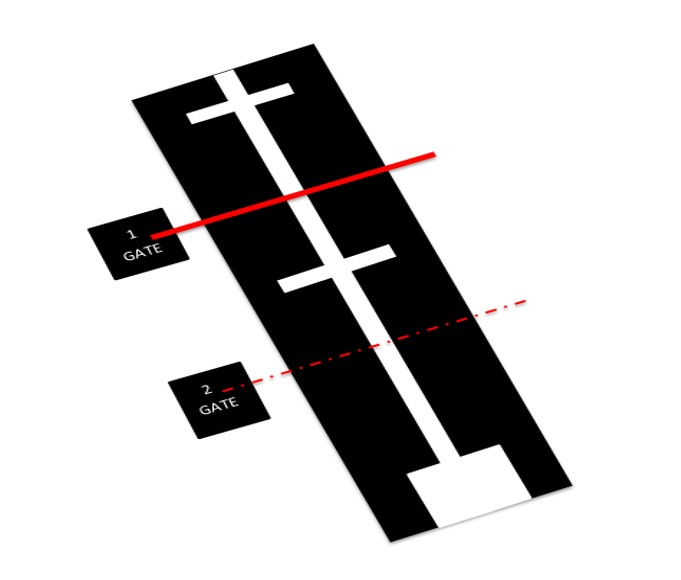
\includegraphics[scale = 0.5]{images/sit1.jpg}
            \caption{Situation 1}
            \label{fig:my_label}
        \end{figure}
        
        In this situation we have to wait until the GATE 1 is opened. If we detect GATE 1 is opened then after 3s the GATE 2 is also opened. Now, both gates are opened for 7s. Therefor we can go to destination with appropriate acceleration.
        
    \subsection*{2.	Second situation $\rightarrow$ if we detect GATE 1 is opened and GATE 2 is closed,}
        \begin{figure}[h]
            \centering
            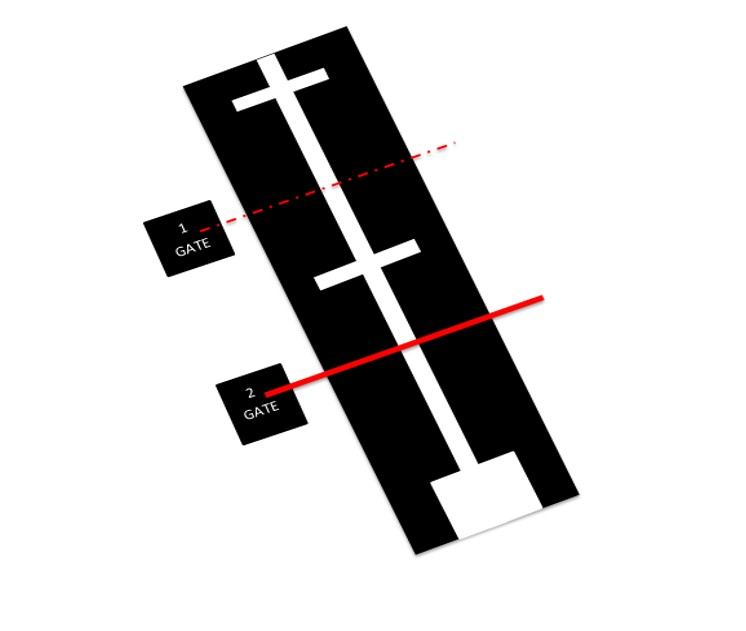
\includegraphics[scale = 0.5]{images/sit2.jpg}
            \caption{Situation 2}
            \label{fig:my_label}
        \end{figure}
        
        In this situation we have to wait maximum 3s. After this time (max -3s) the both GATES are opened for 7s. Therefor we can go to destination with appropriate acceleration. 
    
    \subsection*{3.	Third situation $\rightarrow$ both GATES are opened}
        \begin{figure}[h]
            \centering
            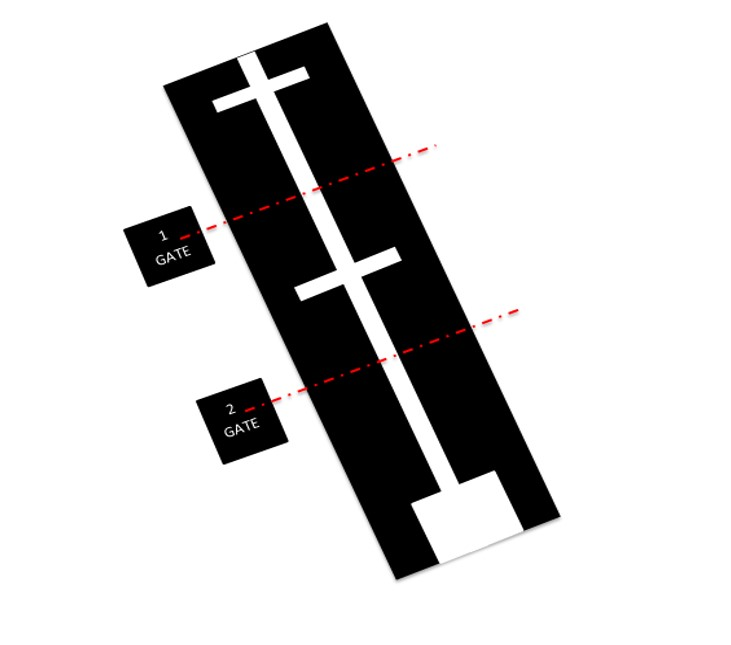
\includegraphics{images/sit3.jpg}
            \caption{Situation 3}
            \label{fig:my_label}
        \end{figure}
        In this situation we have to wait maximum 17s for both gates are opened. After this time (max – 17s) the both GATES are opened for 7s. Therefor we can go to destination with appropriate acceleration.
        \par
        In this final task we can detect the both gates from the first intersection line. Because, distance between 1st intersection line and GATE 1 is nearly 30cm and distance between 1st intersection line and GATE 1 is nearly 90cm. TOF sensor can measure these distance precisely. 
        \par
        According to the above three situations we complete final task when both gates are opened in same time. Therefor we have to choose appropriate acceleration for the robot.
        
        $Minimum \ acceleration = (2 \times 120)/49
                                            = 4.898cms^{-2}  \\          
Therefore, \ we \ have \ to \ maintain \  our\  robot\  acceleration \geq 4.898cms^{-2}$



    

%\printbibliography
\printbibliography


\end{document}
